\section{RESULTADOS PRELIMINARES}

Nesta seção apresentaremos o andamento deste trabalho até o presente momento.

Até o momento, de concluído, temos o processo que está sendo utilizado durante o desenvolvimento do sistema, os requisitos do sistema que já foram coletados, analisados e validados, além do próprio projeto do sistema. 

Na fase que está em andamento, que é a fase de implementação, já temos os seguintes módulos concluídos: 

\begin{alineascomponto}
	\item Gerenciador de Usuários: módulo responsável por gerenciar os usuários do sistema como professores, assistentes e alunos.
	\item Gerenciador de Turmas: módulo responsável por gerenciar as turmas de alunos do sistema.
    \item Gerenciador de Disciplinas: módulo responsável por gerenciar as disciplinas que serão cadastradas no sistema.
    \item Gerenciador de Lições: módulo responsável por gerenciar as lições que os professores irão cadastrar no sistema.
    \item Gerenciador de Questões: módulo responsável por gerenciar os problemas que os assistentes e professores poderão cadastrar para cada lição.
    \item Gerenciador de Pontuação: módulo responsável por gerenciar a pontuação ganha pelos alunos, assim como seu nível de experiência ao longo da utilização do sistema. 
    \item Fórum: módulo responsável por permitir que alunos postem dúvidas dos mais variados  assuntos relacionadas ao sistema, seja dúvidas em relação ao conteúdo apresentado em sala de aula, assim como informações sobre o sistema e sugestões. 
\end{alineascomponto}

Os módulos que ainda restam para serem desenvolvidos nesta fase são:

\begin{alineascomponto}
	\item Gerenciador do Progresso: módulo responsável por acompanhar o andamento de cada aluno durante seu aprendizado, para identificar obstáculos epistemológicos enfrentados pelos alunos para poder assim, alertar o professor, caso o aluno faça parte de alguma turma, ou sugerir que esse aluno peça ajuda ao sistema, para que o sistema envie esse pedido de ajuda a outros alunos que já concluíram aquele conteúdo com certo nível de proficiência.
	\item Chat: quando um aluno enfrentar um obstáculo epistemológico e o sistema sugerir que ele peça ajuda a outros alunos, esse módulo será responsável por mediar a comunicação entre esse aluno com dificuldade e o que se disponibilizar a prestar essa ajuda.
    \item Gerador de Estatísticas: módulo responsável por gerar as estatísticas que o professor utilizará para acompanhar o andamento de suas turmas e alunos, assim como para o uso pelo aluno, que utilizará para acompanhar seu próprio progresso durante sua aprendizagem no sistema.
    \item Ranking: módulo responsável por manter um ranking\footnote{É uma classificação ordenada de acordo com critérios determinados.} com os posicionamentos dos alunos de acordo com seu desempenho no sistema durante a semana.
    
\end{alineascomponto}

A seguir, apresentaremos algumas telas do sistema:

\begin{figure}[H]
  \centering
  \begin{minipage}[b]{0.49\textwidth}
	\caption{Tela Inicial}
    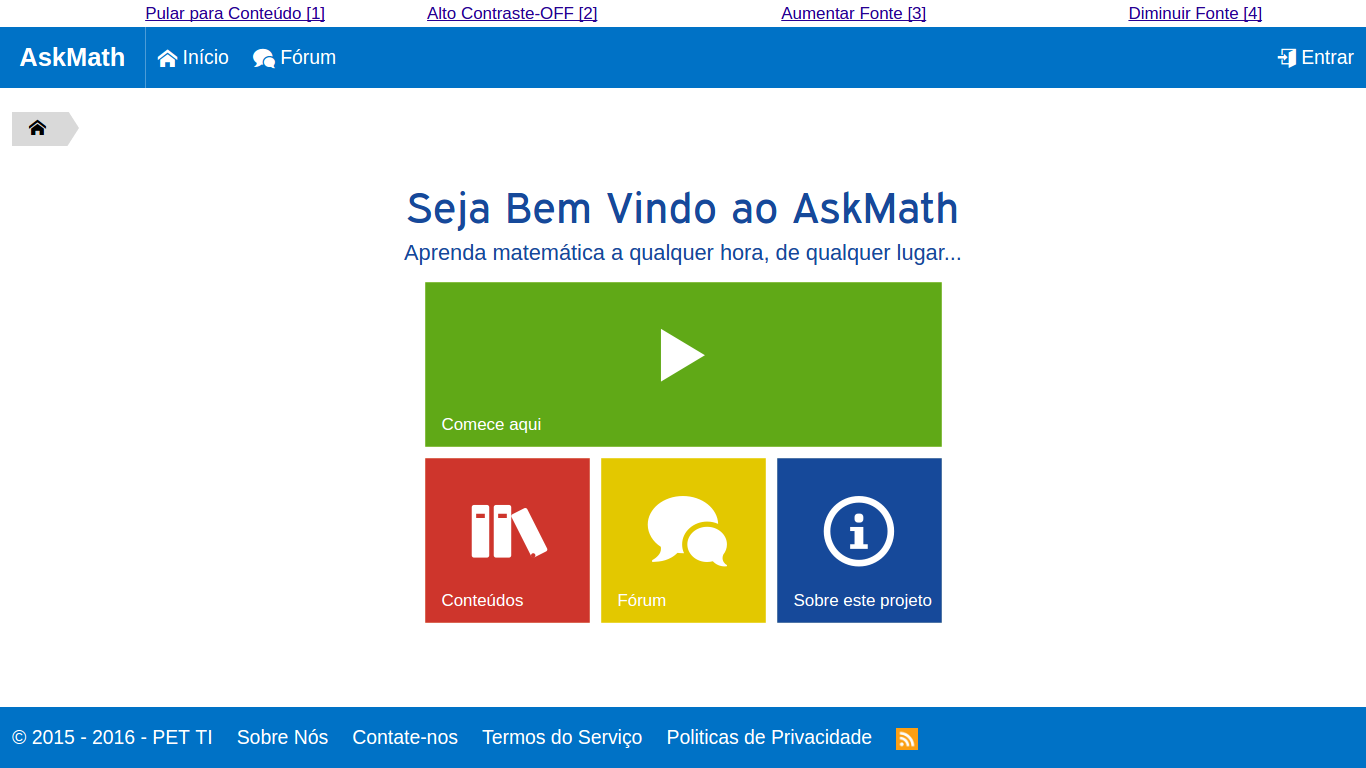
\includegraphics[width=\textwidth]{figuras/askmath/1}
    \\
    \\
  \end{minipage}
  \hfill
  \begin{minipage}[b]{0.49\textwidth}
	\caption{Tela Inicial do Aluno}
    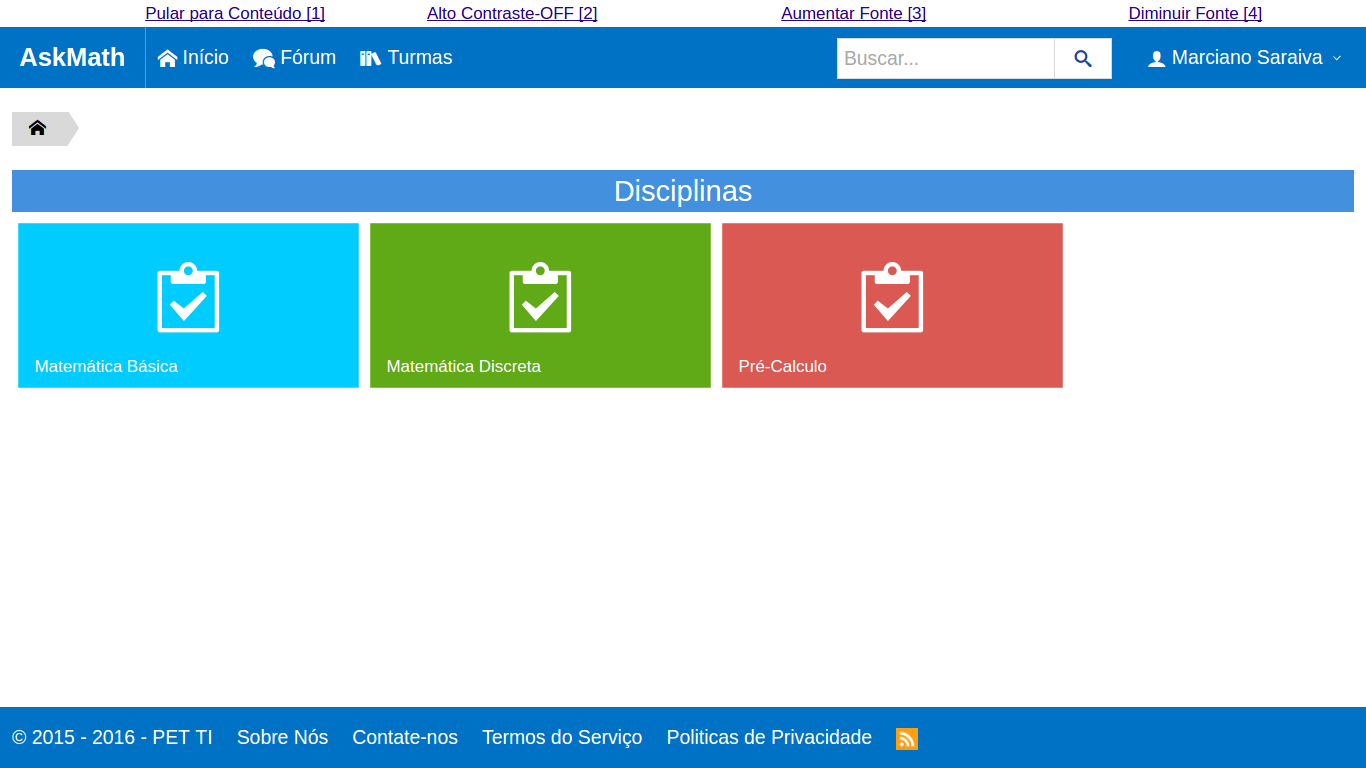
\includegraphics[width=\textwidth]{figuras/askmath/2}
  	\\
    \\
  \end{minipage}
 
  \begin{minipage}[b]{0.49\textwidth}
    \caption{Tela de Administra\c{c}\~ao}
    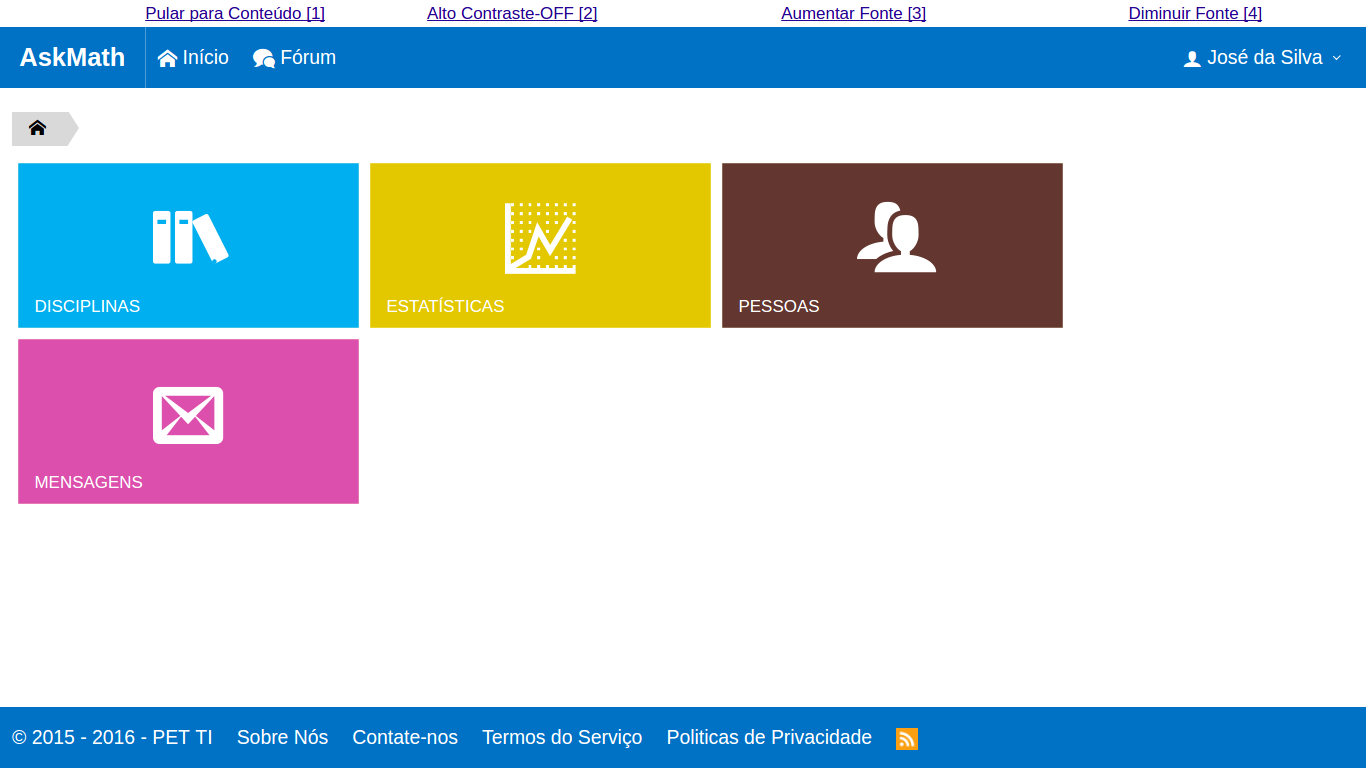
\includegraphics[width=\textwidth]{figuras/askmath/3}
  \end{minipage}
  \hfill
  \begin{minipage}[b]{0.49\textwidth}
	\caption{Tela de Problemas do Aluno}
    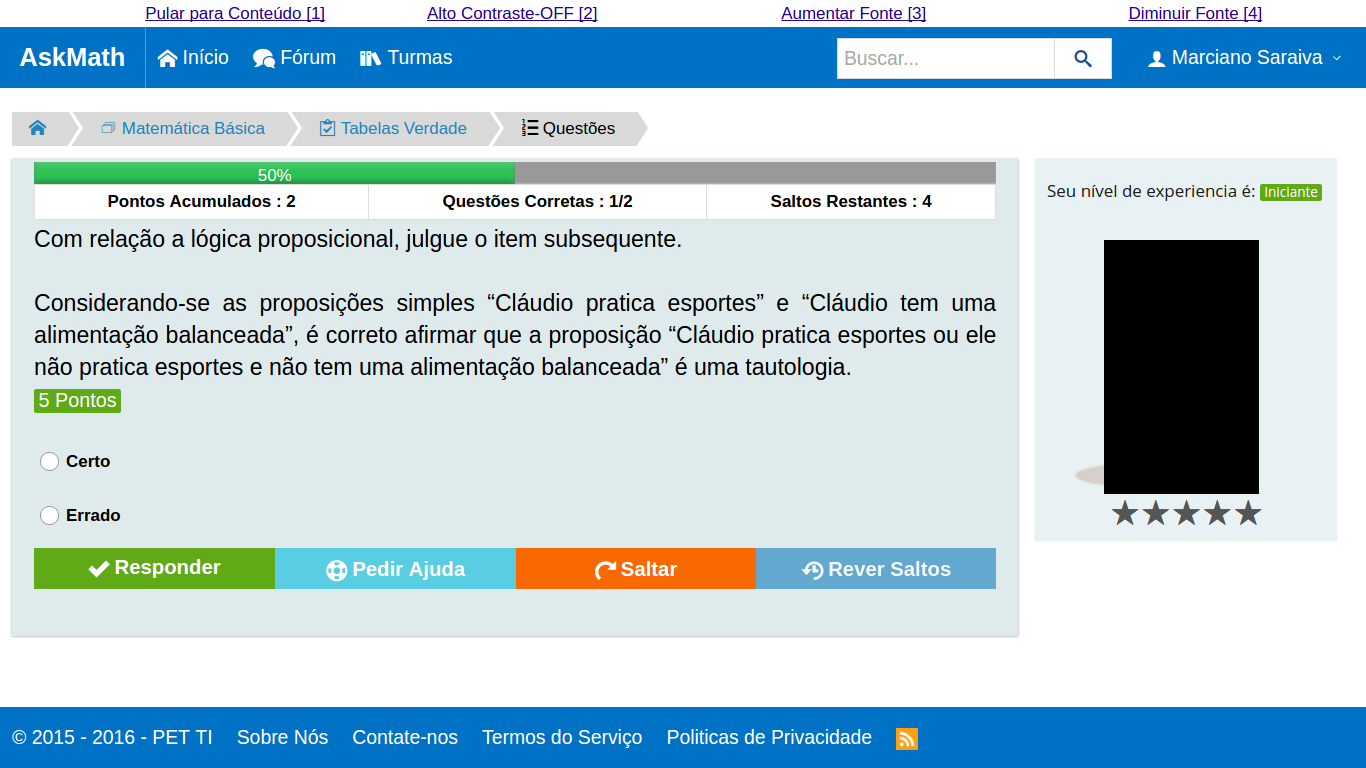
\includegraphics[width=\textwidth]{figuras/askmath/4}
  \end{minipage}
\end{figure}

Os conteúdos que serão utilizados para popular o sistema, durante sua aplicação na UFC-Campus Quixadá, já estão sendo desenvolvidos pelos monitores citados anteriormente. Após a validação e verificação do sistema, esses conteúdos serão adicionados por esses monitores, que passaram por um treinamento para aprenderem a utilizar o sistema.







